\section{はじめに}

我々は,オープンソース脆弱性スキャナであるVuls\cite{vuls}の開発を継続的に行っている.
本稿では,開発過程において直面した主な課題と,それに対する解決アプローチについて論じる.

第一の課題は,MITRE CVE\cite{mitre-cve}やNIST NVD\cite{nist-nvd}といった主要なデータソースにおいて,更新が遅延し,古い情報が長期間残存する場合がある点である.
このため,これらのデータソースを用いて脆弱性を検知した際に,未検知・誤検知が発生することがある.
例えば,CVE-2023-26207はFortinet FortiOSおよびFortiProxyに関する脆弱性である.
影響を受けるプロダクトとして,NIST NVDは図\ref{fig:cve-2023-26207-nvd}のように示しており,Fortinetでは図\ref{fig:cve-2023-26207-fortinet}のように示している.
Fortinetによると,FortiOS 7.0.0から7.0.15までのバージョンは影響を受けるとされているが,NIST NVDでは影響を受けるプロダクトとして示されていない.
つまり,NIST NVDの情報を信頼して脆弱性を検知した場合,未検知が発生する.
したがって,MITRE CVEやNIST NVDのみに依存せず,可能な限りベンダが直接公開するセキュリティアドバイザリなどの一次データソースから脆弱性情報を収集することが極めて重要である.

\begin{figure}[htbp]
    \begin{center}
            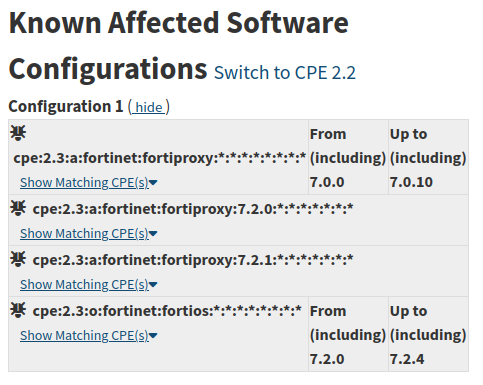
\includegraphics[scale=0.5]{./1-introduction/cve-2023-26207-nvd.png}
            \caption{NIST NVDによるCVE-2023-26207の影響を受けるプロダクト\cite{cve-2023-26207-nvd}}
            \label{fig:cve-2023-26207-nvd}
    \end{center}
\end{figure}

\begin{figure}[htbp]
    \begin{center}
        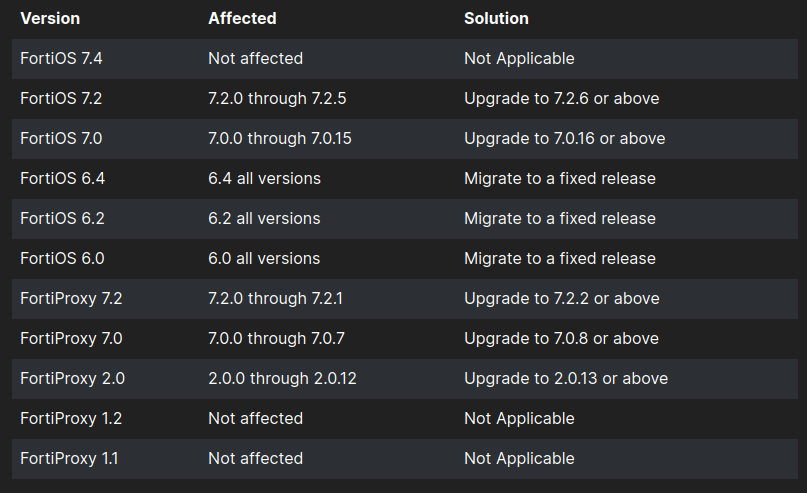
\includegraphics[scale=0.3]{./1-introduction/cve-2023-26207-fortinet.png}
        \caption{FortinetによるCVE-2023-26207の影響を受けるプロダクト\cite{cve-2023-26207-fortinet}}
        \label{fig:cve-2023-26207-fortinet}
    \end{center}
\end{figure}

第二の課題は,脆弱性情報が複数のデータフォーマットで提供されることである.
はじめに,開発者は提供されるそれぞれのフォーマットの仕様を理解することが求められる.
そして,実際に提供されるデータに沿って,さらにベンダ向けの調整が求められる.
例えば,2025年8月時点で,Red Hatは,OVAL形式\cite{redhat-ovalv2}とCSAF/VEX形式\cite{redhat-vex},OSV形式\cite{redhat-osv},CVE形式\cite{redhat-cve}の四つのフォーマットで脆弱性情報を提供している.
まず,開発者はこの4つのフォーマットを理解し,それぞれのフォーマットで記述された脆弱性情報の特徴を把握しなければならない.
OVAL形式は,メジャーバージョン毎に分かれ,未修正な脆弱性情報やExtended Update Supportの情報を含むかなどの観点で,さらに細かく分割されている.
対して,CSAF/VEX形式は,ID毎に提供されており,すべてのプロダクトに対する脆弱性情報が単一のファイルで提供される.
脆弱性と紐付けるパッケージの記述方法も異なる.
OVAL形式は,どのような脆弱性に対してもすべてバイナリパッケージ単位で紐付けるが,CSAF/VEX形式では,修正済みな脆弱性ではバイナリパッケージおよびソースパッケージの両方が紐付けされ,未修正や影響を受けない脆弱性においては,ソースパッケージ単位が紐付けされる\footnote{2025年8月時点で,CSAF/VEX形式において,未修正や影響を受けない脆弱性の場合でもバイナリパッケージ,ソースパッケージの両方を紐付けるように変更が進められている\cite{redhat-secdata-1097}.}.
このような違いにより,スキャナで収集する検知対象の情報や利用するデータフォーマットを適切に選択する必要が生じる.
Red Hatだけでなく,DebianやUbuntuなど多くのディストリビューションで,脆弱性情報が複数のフォーマットで提供されており,開発者にとって非常に負担となっている.
また,このデータフォーマットの違いは,利用者にも負担を与えており,脆弱性を検知するための必要な情報が検知対象毎に異なったり,誤検知を判断するとき,検知対象ごとに採用しているフォーマットと密接に結びついた実装を考慮する必要がある.

第三の課題は,脆弱性検知の再現性の確保や,検知結果の変化理由を説明することの困難さである.
従来は,ベンダから取得した脆弱性情報を直接変換し,脆弱性データベースを構築していた.
しかし,この方法では,例えばサーバーダウン等によりベンダから情報が取得できない場合,脆弱性データベースの更新が不可能となる.
また,誤検知の報告を受けた際,報告者が利用した脆弱性データベースを共有してもらわなければ,問題の再現や調査が困難であった.
さらに,検知結果に変化が生じた場合,たとえば以前検知されていた脆弱性が検知されなくなった場合,その理由を説明するためには,過去と現在の脆弱性データベースを比較する必要があるが,利用者が適切にデータベースを履歴管理していることは非常に稀である.

本研究では,これらの課題を解決するために以下の3点を達成する仕組みを提案し,評価する.
\begin{itemize}
    \item 一次データソースの情報をできる限り幅広く収集・採用することで,脆弱性情報の鮮度を保ち,未検知や誤検知のリスクを低減する.
    \item 収集した脆弱性情報を共通データ構造に変換することで,多くの開発者や利用者は脆弱性情報を一貫した形式で扱うことができ,異なるフォーマットの違いを意識する必要がなくなる.
    \item 収集したデータソースと共通データ構造に変換された脆弱性情報を履歴管理し、それらをもとに脆弱性データベースを構築することで,再現性や説明性,運用効率の向上を図る.
\end{itemize}